\documentclass{article}
\usepackage{tikz}

\begin{document}

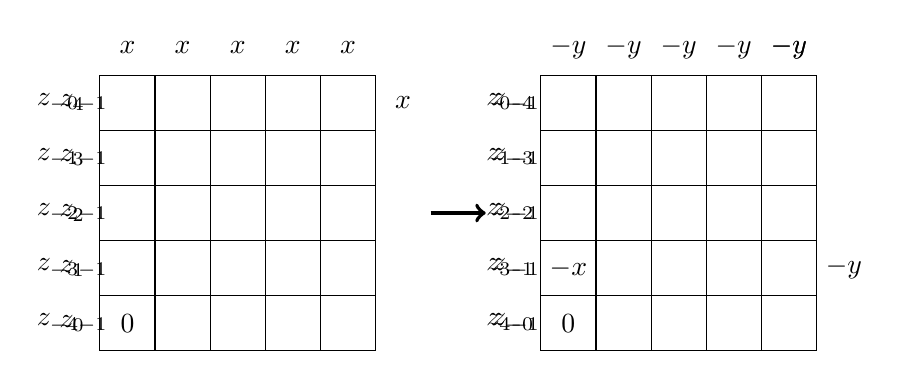
\begin{tikzpicture}[scale=0.7]
    % Draw the first grid
    \draw[step=1cm, black, thin] (0, 0) grid (5, 5);
    
    % Add labels to the first grid
    \foreach \i in {0,1,2,3,4} {
        \node at (-0.5, \i+0.5) {\(z_{\i}\)};
        \node at (\i+0.5, 5.5) {\(x\)}; % Only top middle for x in the first grid
        \node at (-0.5, 4.5-\i) {\(z_{-\i-1}\)}; % Negative indices
    }
    \node at (0.5, 0.5) {\(0\)}; % Center bottom left at (0.5,0.5)
    \node at (5.5, 4.5) {\(x\)}; % Top right corner for the first grid
    
    % Draw an arrow to indicate transformation
    \draw[->, line width=0.5mm] (6, 2.5) -- (7, 2.5);
    
    % Draw the second grid
    \draw[step=1cm, black, thin] (8, 0) grid (13, 5);
    
    % Add labels to the second grid
    \foreach \i in {0,1,2,3,4} {
        \node at (7.5, \i+0.5) {\(z_{-\i}\)};
        \node at (7.5, 4.5-\i) {\(z_{\i-1}\)}; % Adjusted negative indices
        \node at (8+\i+0.5, 5.5) {\(-y\)}; % Only top middle for -y in the second grid (example at top right)
    }
    % Correcting the label placements specifically for clarity
    \node at (8.5, 0.5) {\(0\)}; % Center bottom left at (8.5,0.5)
    \node at (13.5, 1.5) {\(-y\)}; % Example label for -y at specific position
    \node at (12.5, 5.5) {\(-y\)}; % Example label at the top right of the second grid
    
    % Additional specific labels
    \node at (8.5, 1.5) {\(-x\)}; % Example label for -x in second grid
\end{tikzpicture}

\end{document}